\documentclass[a4paper,ngerman,british,BCOR1.5cm,headsepline,DIV12,appendixprefix,final]{scrbook}

\usepackage[utf8x]{inputenc}
\usepackage{ucs}
\usepackage[OT1]{fontenc}
\usepackage{babel}

\usepackage{varioref}
\usepackage[pdftex,plainpages=false,pdfpagelabels=true,pdfusetitle]{hyperref}
%              citebordercolor={0.75 0.75 1},
%              filebordercolor={0.75 0.75 1},
%              linkbordercolor={0.75 0.75 1},
%              pagebordercolor={0.75 0.75 1},
%              urlbordercolor={0.75 0.75 1},
%              pdfborder={0.75 0.75 1},
\usepackage[all]{hypcap}
\usepackage{graphicx}
\usepackage{subfigure}
\usepackage{tocvsec2}
\usepackage{engord}
\usepackage{hyphenat}
\usepackage{booktabs}
\usepackage{overpic}
\usepackage{tikz}
\usepackage{rotating}

\usetikzlibrary{positioning}
\usepackage[left,pagewise,modulo,]{lineno}
%\linenumbers


\newcommand{\todo}{\footnote}
\newcommand{\comment}[1]{}

\tolerance 2414
\hbadness 2414
\emergencystretch 1.6em
%\hfuzz 0.3pt
\widowpenalty=10000     % Hurenkinder
\clubpenalty=10000      % Schusterjungen
%\vfuzz \hfuzz
%\raggedbottom


%tocloft fixups
\makeatletter
\providecommand{\IfPackageLoaded}[2]{\@ifpackageloaded{#1}{#2}{}}
\providecommand{\IfElsePackageLoaded}[3]{\@ifpackageloaded{#1}{#2}{#3}}
\makeatother

\IfElsePackageLoaded{subfig}
	% IF subfig
	{\usepackage[subfigure]{tocloft}}{
	% ELSE
	\IfElsePackageLoaded{subfigure}
		% IF subfigure
		{\usepackage[subfigure]{tocloft}}
	   % Else (No subfig nor subfigure)
		{\usepackage{tocloft}}
	}
\IfPackageLoaded{subfig}{
	\setcounter{lofdepth}{2}
	\setcounter{lotdepth}{2}
}
%tocloft fixups end

\begin{document}
\subject{\LARGE{Salespoint 2011}}
%\title{Implementierung des DDEKit-Ansatzes auf Linux}
%\title{Implementation of the DDEKit approach for Linux.}
%\title{DDEKit-Linux: improved security and ease of development for Linux user space drivers.}
\title{Technical Overview}
\author{Hannes Weisbach}

\publishers{Dresden University of Technology\\
				Faculty of Computer Science\\
				Institute of Software- and Multimedia- Technology\\
				Professorship of Software Technology\\
\vskip 6cm
\hangafter=0
\footnotesize
	\begin{tabular}{ll}
 		Address                                        & Telephone: 0351 463 38442 \\
		Faculty of Computer Science                    & Fax: 0351 463 38459\\
		Insitute of Software and Multimedia Technology & birgit.demuth@tu-dresden.de\\
		TU Dresden                                     & http://tu-dresden.de\\
		01062 Dresden                                  & \\
	\end{tabular}
}

%\comment{

\hypersetup{
    pdfkeywords={salespoint, swt, praktikum},
    pdfsubject={Salespoint 2011 - Technical Overview},
}

\maketitle

\selectlanguage{british}
\cleardoublepage{}

\maxtocdepth{section}
\tableofcontents{}
\clearpage

\listoffigures
\listoftables

\clearpage

\settocdepth{chapter}
\chapter{Introduction}
The Salespoint Framework is intended to minimize developing effort of e-commerce solutions and point-of-sale applications.
Salespoint 2010 users complained about complexity, missing features and bugs.
Thus, the decision was made to re-design and re-implement the framework from scratch.
Our development goal was an easy-to-use framework primarily targeted for educational purposes.
As such, Salespoint 2011 is not taylored to any specific application, but designed with a wide area of applications in mind.

Models and design patterns employed in Salespoint 2011 are inspired by ``Enterprise Patterns and MDA: Building Better Software with Archetype Patterns and UML'' \cite{MDA} by Jim Arlow.
An overview over the functionality of and new features in Salespoint 2011 is detailed in this document.

We would like to thank all Salespoint users who submitted their feedback and encourage future users of Salespoint 2011 to do the same.

\settocdepth{section}
\chapter{Technical Background}
One of the main reason to use a framework such as Salespoint for educational purposes is to teach students reusability.
The \salespoint{} developers also adhere to that principle.
Thus, \salespoint{} itself uses a number of frameworks and APIs, which are introduced briefly.
The software architecture of \salespoint{} applications is also detailed.
\section{JPA - Java Persistence API}
\label{sec:jpa}
%The persistence layer was one of the biggest problems in Salespoint 2010. We wanted a solution that acknowledges latitudes for persisting objects with relatively low effort.
One of the key features of \salespoint{} is its integrated persistence layer. The goal is to allow data persistence, while minimising programming effort and training period as well as maximising flexibility for framework users.

%Therefore and because of the huge community support, we decided to use the Java Persistence API (JPA). JPA is a Java Programming Language Framework managing relational data in applications. The API itself is defined in the javax.persistence package.
The obvious choice was the Java Persistence API (JPA), a Java framework managing relational data in Java Standard Edition or Enterprise Edition applications. \salespoint{} uses JPA 2.0, developed under JSR 317 and finalised in Dec, 2009 \cite{jpa}.

Additionally to the API itself, which is defined in the \texttt{javax.persistence} package, JPA also consists of \textit{Persistence Entities}, \textit{ORM Metadata} and the \textit{Java Persistence Query Language} (JPQL).

A persistence entity is usually a \textit{Plain Old Java Object} (POJO), which is mapped to a single table in a database.
A row in such a database table corresponds to a specific instance of such an entity.
Relational data between entities (and therefore tables) may be specified in an XML descriptor file or as annotations in Java source code.
\salespoint{} uses annotations to provide object/relational metadata.

Persistence entities may be related to each other by an inheritance hierarchy.
A persistence entity may have a non-persistent superclass.
Fields declared by a non-persistent superclass are not stored in the database if an inheriting entity is persisted.
Three schemes exist to persist entites with an inheritance relationship: \textit{single table}, \textit{join table}, and \textit{table per class}.

The \textit{single table} strategy stores all instances of classes of an inheritance hierarchy in the same table.
The table contains columns for every attribute a persistence entity in the hierarchy declares.
The different types are distinguished by a type discriminator column.
The discriminator value for each persistence entity in an inheritance hierarchy is generated automatically or can be supplied by the user.

The \textit{join table} strategy uses a table for the root persistence entity of the inheritance hierarchy.
Additionally, a table is addded for each persistence entity in the inheritance hierarchy.
In the supplementary tables, a foreign key is used to reference a row in the table of the parent persistence entity.
Each table contains only columns for fields declared by a specific persistence entity in the inheritance hierarchy, but neither for the entities children nor parents.
To reconstruct an object from the database, the different tables have to be joined using this foreign key, thus the name of this strategy.

The \textit{table per class} strategy creates a table for each persistence entity containing all fields of the class, including inherited fields.

The inheritance strategy of an inheritance hierarchy has to be declared at the root persistence entity.
The inheritance stratety may not be changes for a sub-hierarchy, because JPA 2.0 does not require this feature.
JPA 2.0 only requires the \textit{single table} and \textit{join table} strategies to be implemented.
\salespoint{} uses the \textit{single table} strategy exclusively.

The query language JPQL, which is similar to SQL, is used to retrieve entity information from the database.
In contrast to SQL, JPQL queries act on entity objects instead of database tables.
JPA implementations translate a JPQL statement to SQL statements at run time.
It is possible to replace the DBMS while keeping the Java classes.
It is possible to interface directly with the DBMS using \textit{Native Queries}.
\salespoint{} however, uses the \textit{Criteria API} \cite{jpa, eclipselink-javadoc} to facilitate type safe querying.

%Some of the most popular vendors of JPA are Hibernate and EclipseLink. For developing Salespoint 2011 we used JPA 2.0 with EclipseLink without vendor specific functionality. So it should also be possible to use other JPA 2.0 vendors like Hibernate with this framework.
Multiple implementations of JPA 2.0 exist, for example TopLink \cite{toplink} and EclipseLink \cite{eclipselink}.
The open source persistence and ORM framework Hibernate \cite{hibernate} also supports JPA 2.0.
\salespoint{} uses the JPA 2.0 reference implementation, EclipseLink.
No implementation specific code is used in \salespoint{}, therefore it should be possible to interchange EclipseLink with another JPA 2.0 implementation.\footnote{This document will be updated, as soon as another JPA provider is tested with \salespoint{}.}

\section{Joda Time}
Joda Time~\cite{jodatime} is a Java date and time API.
It provides a quality replacement for the Java date and time classes.
%We used this API because the Java Date and Calendar classes are badly designed.
\salespoint incorporates Joda Time, because it is open source, easy to use and offers better performance characteristics than Java date and time classes.

Key concepts from Joda Time used in \salespoint{} are \textit{Instant}, \textit{Interval}, \textit{Duration} and \textit{Period}.
From Joda Time documentation:
\begin{quote}
The most frequently used concept in Joda-Time is that of the \textit{instant}.
An Instant is defined as \textit{an instant in the datetime continuum specified as a number of milliseconds from 1970-01-01T00:00Z}.
This definition of milliseconds is consistent with that of the JDK in \code{Date} or \code{Calendar}.
Interoperating between the two APIs is thus simple.
\end{quote}

\textit{Intervals} are defined by two Instants.
An Interval is \textit{half-open}, that is to say the start is inclusive but the end is not
Also, the end is always greater or equal than the start.

\textit{Durations} in Joda Time represent a duration in time, exact to the milisecond.
Durations can be thought of as length of an Interval.

\textit{Periods} also represent durations in time, but in a more abstract way
A Period may be a month, which may be 28, 29, 30 or 31 days, thus the length in miliseconds of those periods differ.

If you, for example have an Instant of February, 1st and add a Period of one month, the result will be an Instant of March, 1st.
Adding instead a Period of 30 days to an Instant of February, 1st will result in an Instant of March, 2nd or March 3rd, depending if the Instant is in a leap year or not.

\section{Spring}
In contrast to earlier versions of the Salespoint Framework, \salespoint{} obeys the MVC pattern. 
\salespoint{} can be seen as the Model of an MVC application, no parts of the View or the Controller are incorporated in the Framework.

\salespoint{} is designed as basis for development of web applications, using the \textit{Spring Framework}~\cite{spring} to implement Views and Controllers.
To further ease the development, \salespoint{} includes property editors to convert string based representations to \salespoint{} identifier types.
Also, JSP tags to check if a user is logged in and if a user has a certain capability are included in the framework.

\section{Software Architecture of a \salespoint{} Application}
Software often need to be adaptive, flexible, and extendable.
Using a suitable architecture pattern, such as the Model-View-Controller pattern, helps to meet these non-functional requirements.
Figure \ref{sp5-arch} gives an overview of how a \salespoint{} application is modelled.
\salespoint{}, as domain framework, takes the place of the model in the MVC pattern.
The model can be extended by sub-classing \salespoint{} classes or by introducing entirely new classes.
\salespoint{} model classes and sub-classes thereof are transparently stored in a database.
If new classes are added to the model and their state is also required to be persistent, the developer also has to facilitate persisting those objects using the JPA-API.

\begin{figure}[ht]
	\centering
  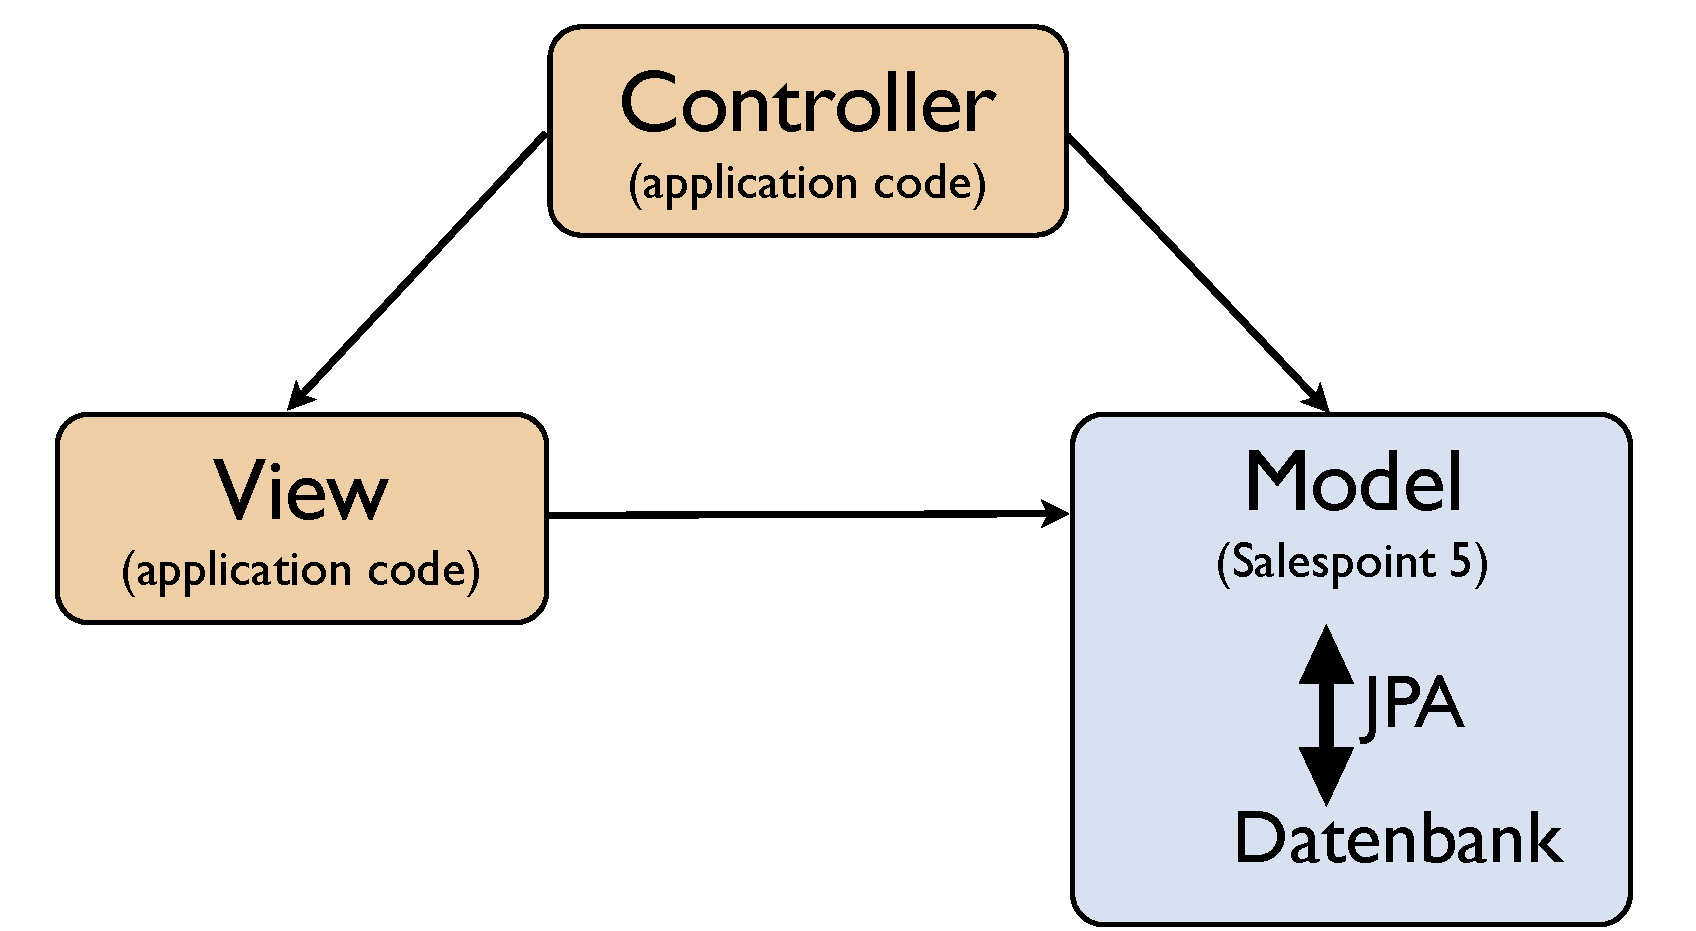
\includegraphics[width=0.6\textwidth]{images/sp5-arch.pdf}
	\label{sp5-arch}
	\caption{MVC-pattern of a \salespoint{} application divided into application specific code (red) and framework code (blue).}
\end{figure}

The controller and view are application-specific and have to be implemented by the user.
Although \salespoint{} does not require a specific framework or API like Swing~\cite{swing} or SWT~\cite{swt}.
However, because \salespoint{} is intended to be used in conjunction with the Spring MVC~\cite{spring} framework for SWP at TU Dresden, \salespoint{} contains supplementary code, easing the development of Spring applications.
This supplementary code consists of Spring MVC \code{PropertyEditor}s, and custom, \salespoint{} specific JSP-tags.
\\

\begin{figure}[ht]
	\centering
  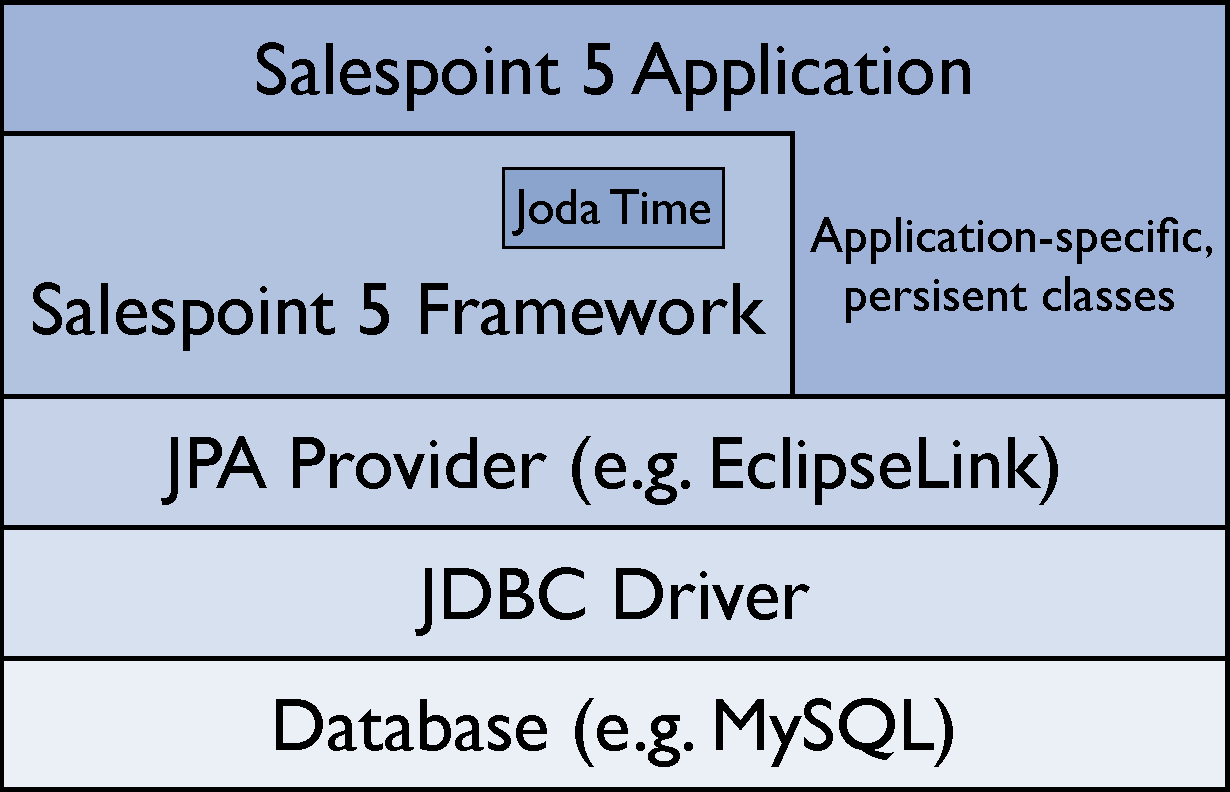
\includegraphics[width=0.45\textwidth]{images/sp5-layered.pdf}
	\label{sp5-layered}
	\caption{TODO}
\end{figure}
A layered view of the software architecture of a \salespoint{} application is shown in Figure \ref{sp5-layered}.
The bottom layer corresponds to a DBMS, chosen by the developer.
As stated in Section \ref{sec:jpa}, JPA works with every DBMS for which a JDBC driver is available.
The JPA provider, which is also chosen by the developer, interfaces with the JDBC driver and \salespoint{}.
\salespoint{} in turn uses a class library, namely Joda Time~\cite{jodatime}, to deal with dates and times.


\newpage
\chapter{\salespoint Core}
This chapter overviews the core functionality of \salespoint and gives a short introduction.
\section{Package Overview}
The following diagram shows the most important packages of the Salespoint 2011 and their dependencies. These and more packages are detailed in the chapters below.

\vskip 1cm

\begin{figure}[ht]
	\centering
  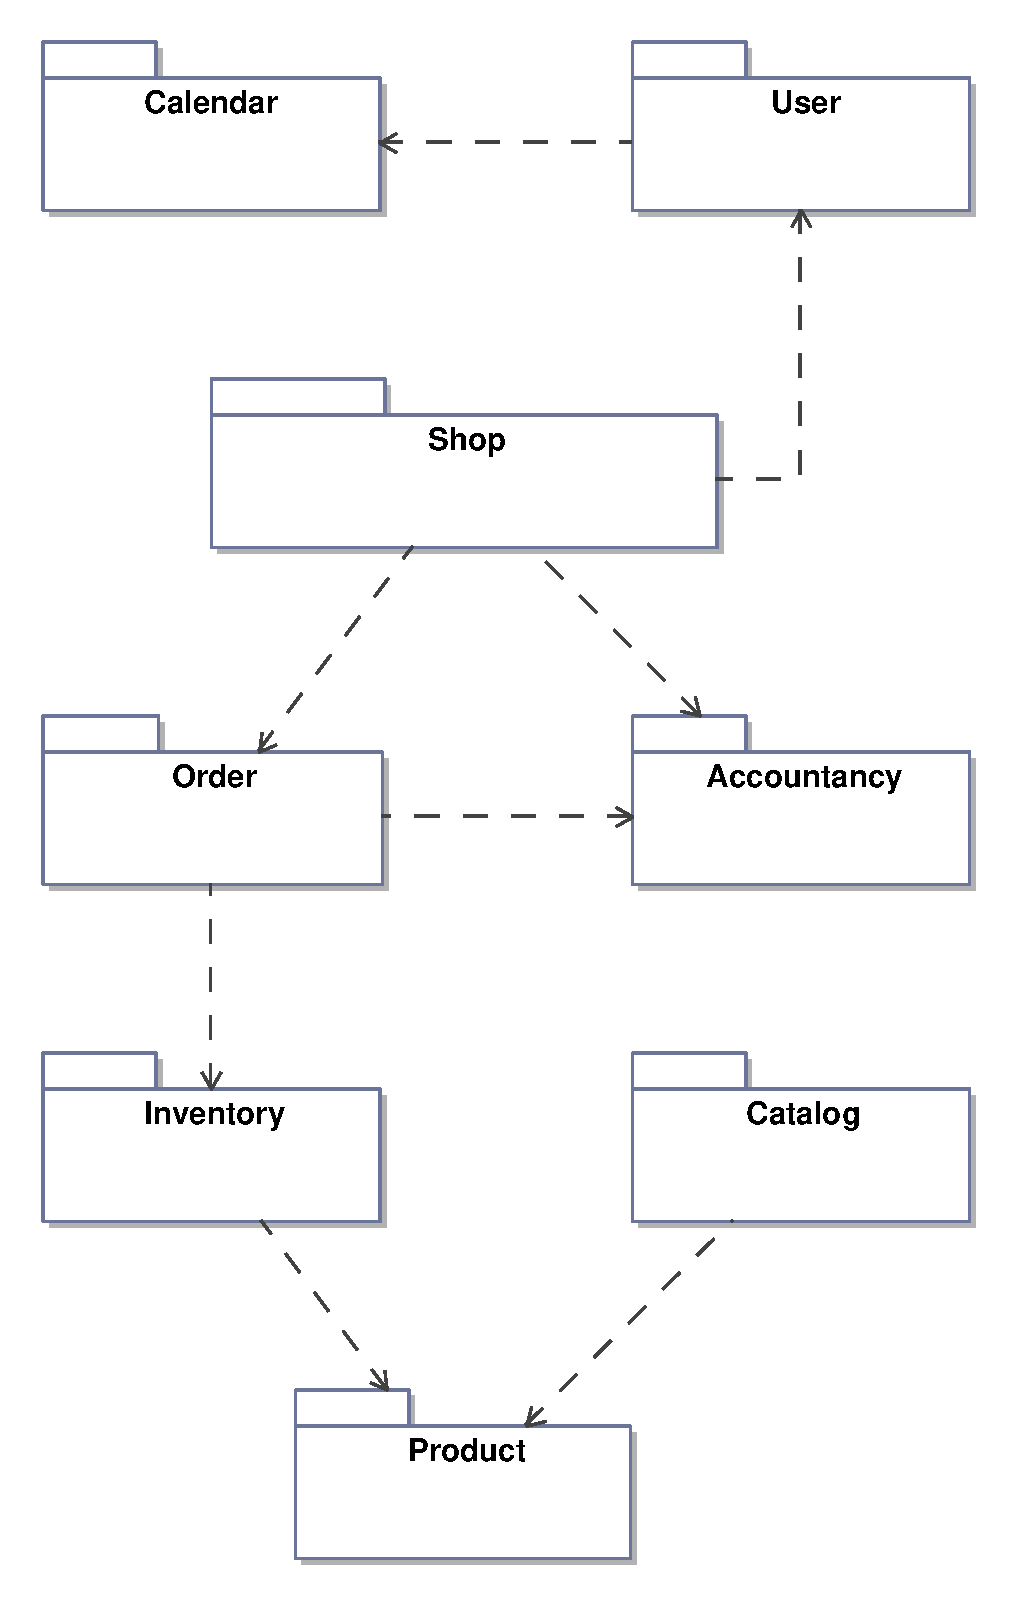
\includegraphics[scale =.45]{images/Overview_Package.eps}
	\label{package_overview}
	\caption{Package Overview}
\end{figure}
\section{Shop}
\label{shop}

\begin{figure}[ht]
	\centering
  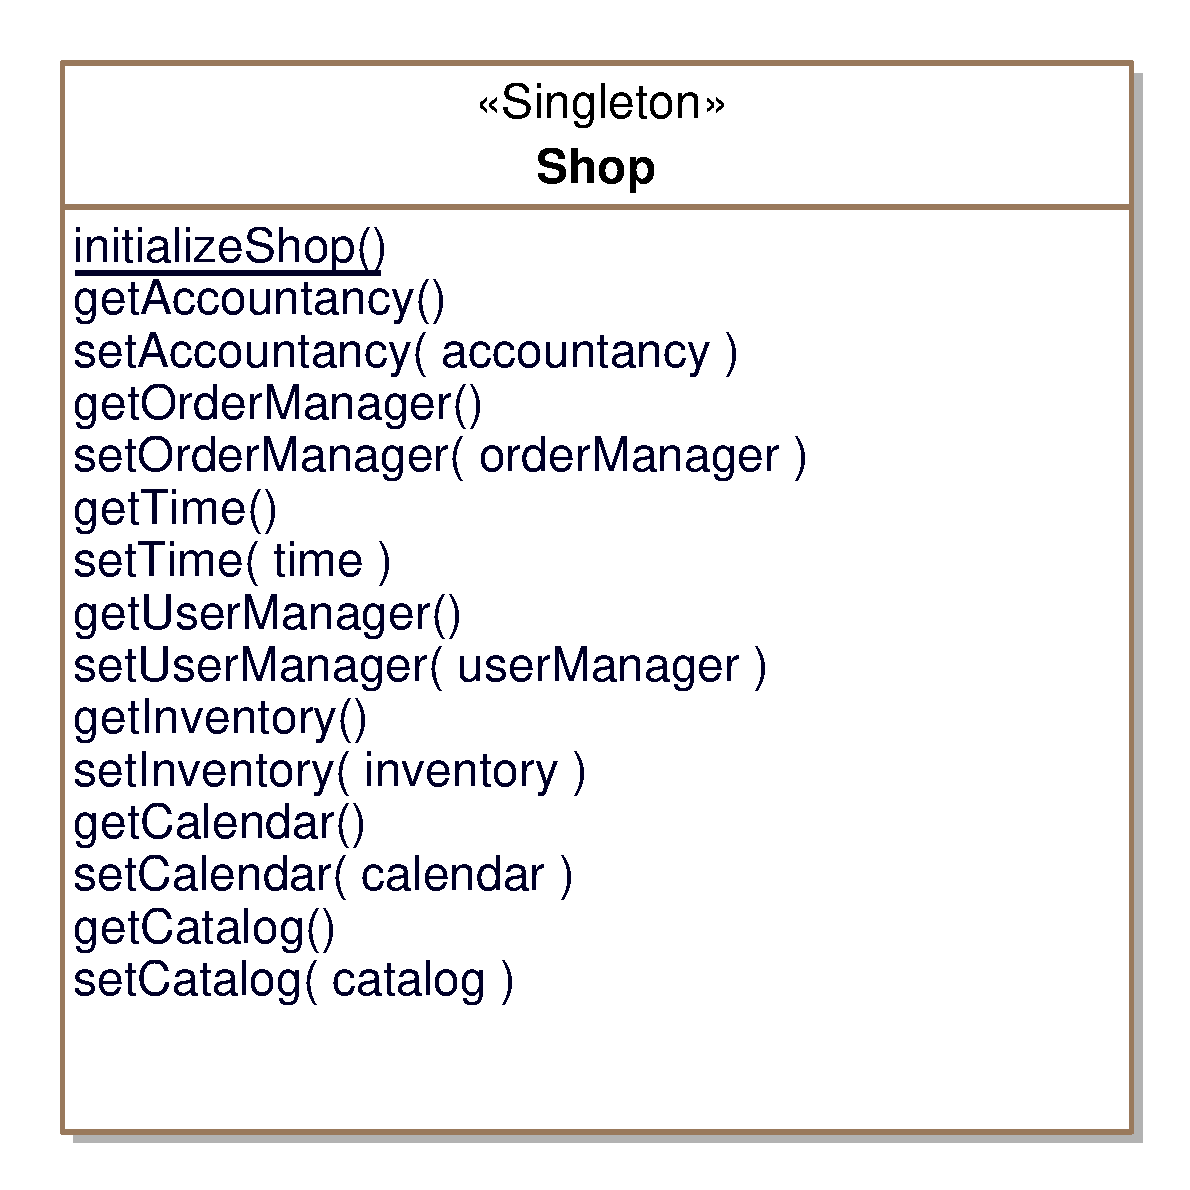
\includegraphics[width=0.65\textwidth]{images/Shop_Overview.eps}
	\label{shop_overview}
	\caption{Shop - Class Overview}
\end{figure}

%\subsection{\code{Shop} - Starting your SalesPoint-application}
\code{Shop} is a central class in \salespoint{}, it holds references to all manager classes and a reference to an implementation of the \code{Time} interface.
There are six manager classes in \salespoint{}: PersistentAccountancy, PersistentCalendar, PersistentCatalog, PersistentInventory, PersistentOrderManager and PersistentUserManager.
Other classes use the \code{Shop} to access the manager classes, for example \code{Order.completeOrder()} uses \code{Shop.INSTANCE.getInventory()} for product removal.
\code{PersistentCalendar} uses \code{Shop.INSTANCE.getTime()} for time based operations.
There is also a convenience method to minimize boilerplate code \code{Shop.initializeShop()}, it's used for setting all managers of \code{Shop} to Salespoints persistent class implementations and the time to \code{DefaultTime}.
\code{Shop} is implemented as singleton.
\newpage
\section{User}

\subsection{How does it works?}

In the Salespointframework there is one \code{PersistenceUsermanger}, but it is not a singelton. You can instanciet a new
\code{PersistenceUsermanger} whenever you need it (it allways manages the same data!).
The Usermanger ist the main part of the UserPackage. It connects all parts:
You can adds and removes User to/from the System and also adds and removes \code{UserCapabilities} of the Users in the System

\begin{figure}[ht]
	\centering
  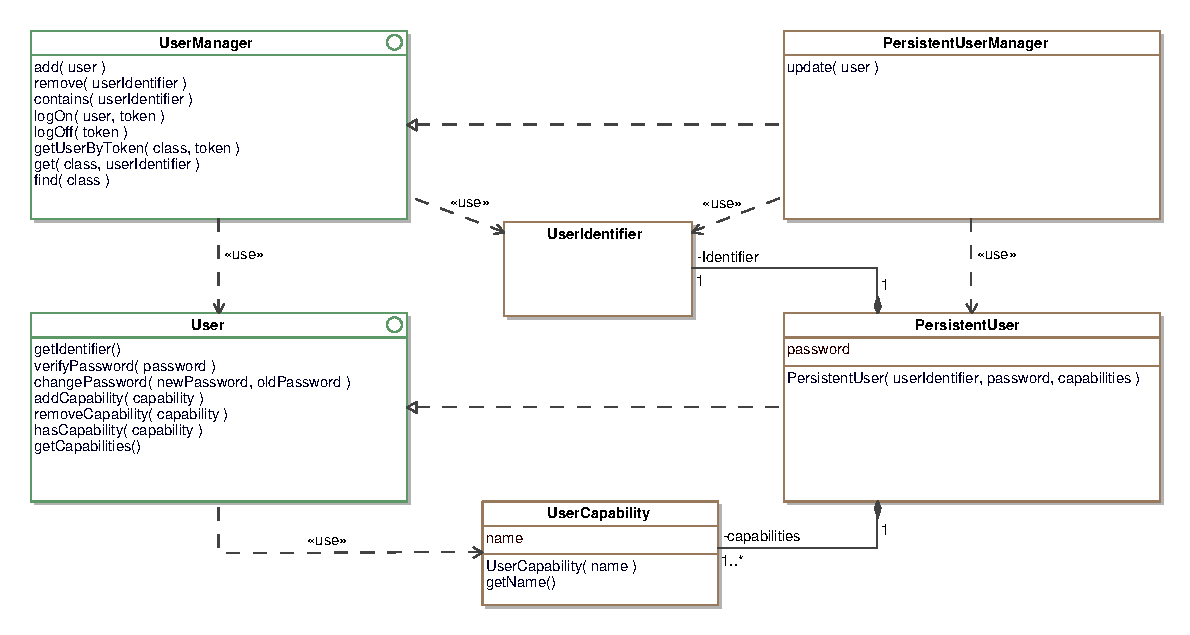
\includegraphics[width=1.0\textwidth]{images/User_Overview.eps}
	\label{user_overview}
	\caption{User - Class Overview}
\end{figure}

\subsection{Ensure correct Data}
To ensure you have the correct data in your system you should only access \code{users} and their \code{UserCapabilities} via the \code{PersistenceUsermanger}:

During the process of adding a user to the system the \code{PersistenceUsermanger} garanties that there will be no duplicate Users. If you try to add a \code{User} with an \code{UserIdentifier} that is already in the system a DuplicateUserException will be thrown. This will help you to identifie \code{Users} correctly, e.g. during the login process.

You should notice that it is not possible to remove Users with open \code{orders}! You have to close/finish them before.

You only able to add a \code{UserCapability} to an \code{user}, which is in they system. Otherwise you will get an UnknownUserException.
This ensures that a new \code{user} will have no \code{UserCapabilities}.

\subsection{Why are there so many users?}
First of all we do have the \code{User} class. This is the user interface with all basic methodes. The are implemented in the
\code{PersistenceUser} and also the basic attributes of an user.
The subclasses of the \code{PersistenceUser} are the \code{AbstractEmployee} and the \code{AbstractCustomer}.
\code{AbstractEmployee}: A spezial User who also has an salary. This helps to work together with the \code{Accountency}.
\code{AbstractEmployee}: This Class is not very usefule, also is shows the user of the Framework that there could be different subclasses of the \code{PersistenceUser}.


\subsection{login}

ASK PAUL!






\newpage
\section{Calendar}
\label{sec:calendar}

The calendar is a new feature in \salespoint{} to manage appointments.
Figure \ref{calendar_overview} shows the UML model of the calendar.

\begin{figure}[ht]
	\centering
  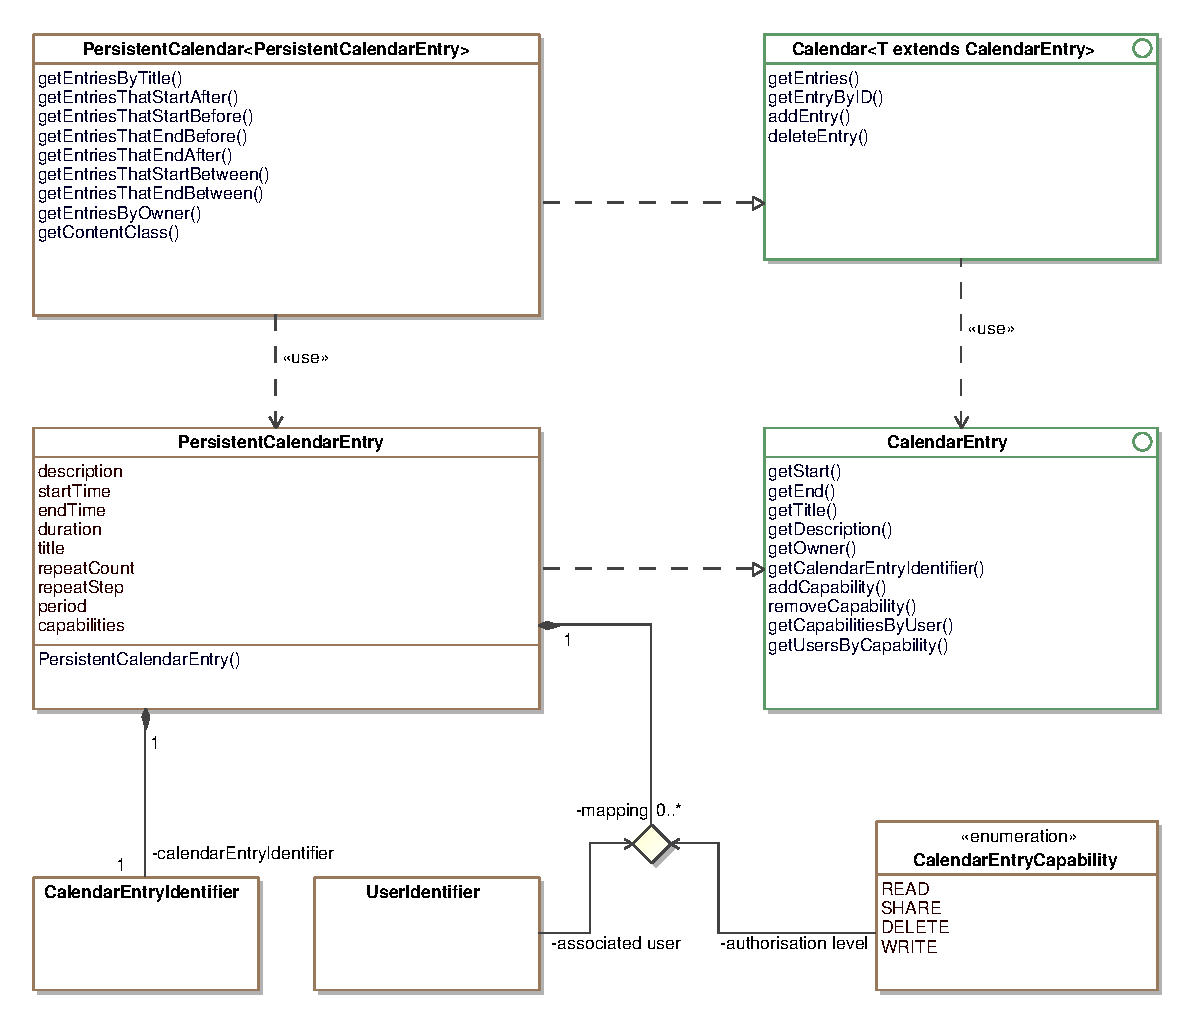
\includegraphics[width=1.0\textwidth]{images/Calendar_Overview.eps}
	\label{calendar_overview}
	\caption{Calendar - Class Overview}
\end{figure}

\code{Calendar} is an interface that provides simple functionality to store calendar entries and retrieve \code{CalendarEntries}.
\code{CalendarEntry} is an interface to set, store and access information about a single appointment.
Both interfaces are implemented by \code{PersistentCalendar} and \code{PersitentCalendarEntry}, respectively.
\code{PersistentCalendarEntry} is a persistence entity containing all information and \code{PersistentCalendar} manages the JPA access.
\\

Every calendar entry is uniquely identified by a \code{CalendarEntryIdentifier}.
This identifier also serves as primary key attribute when persisting an entry to the database.
Additionally, a \code{PersistentCalendarEntry} must have an owner, a title, a start and an end date.
The user who created the entry is known as the owner.
\\

The access of other users than the owner to a calendar entry is restricted by capabilities.
For each calendar entry, a user identifier and a set of capabilities are stored.
Possible capabilities are:
\begin{itemize}
    \item \code{READ} - indicates if a user can read this entry
    \item \code{WRITE} - indicates if a user can change this entry
    \item \code{DELETE} - indicates if a user can delete the entry
    \item \code{SHARE} - indicates if a user can share the entry to other users
\end{itemize}.

Because \salespoint{} only implements the Model, the developer has to check and enforce capabilities in the controller.
\\

Besides the minimum information a calendar entry can also have a description, which may contain more information.
Periodic appointments are also supported, by specifing the number of repetitions and a time span between two appointments.
\\

There are some conditions for temporal attributes of an calendar entry:
\begin{itemize}
    \item the start must not be after the end
    \item the time between two repetitions of an appointment need to be longer than the appointment, so appointments do not overlap
\end{itemize}
%All attributes of the entry can be changed, except of the owner, who will be defined when the entry is created and then becomes immutable. 

\newpage
\section{Quantity}
\code{Quantity} is used to represent amounts of anything.
Three attributes allow \code{Quantity} to specify everything: a numerical value (\code{BigDecimal}), a (measurement) unit or metric (\code{Metric}), and a type specifying the rounding of the numerical type (\code{RoudingStrategy}).

\code{Quantity} objects are immutable and the class implements the \code{Comparable} interface.

\begin{figure}[ht]
	\centering
  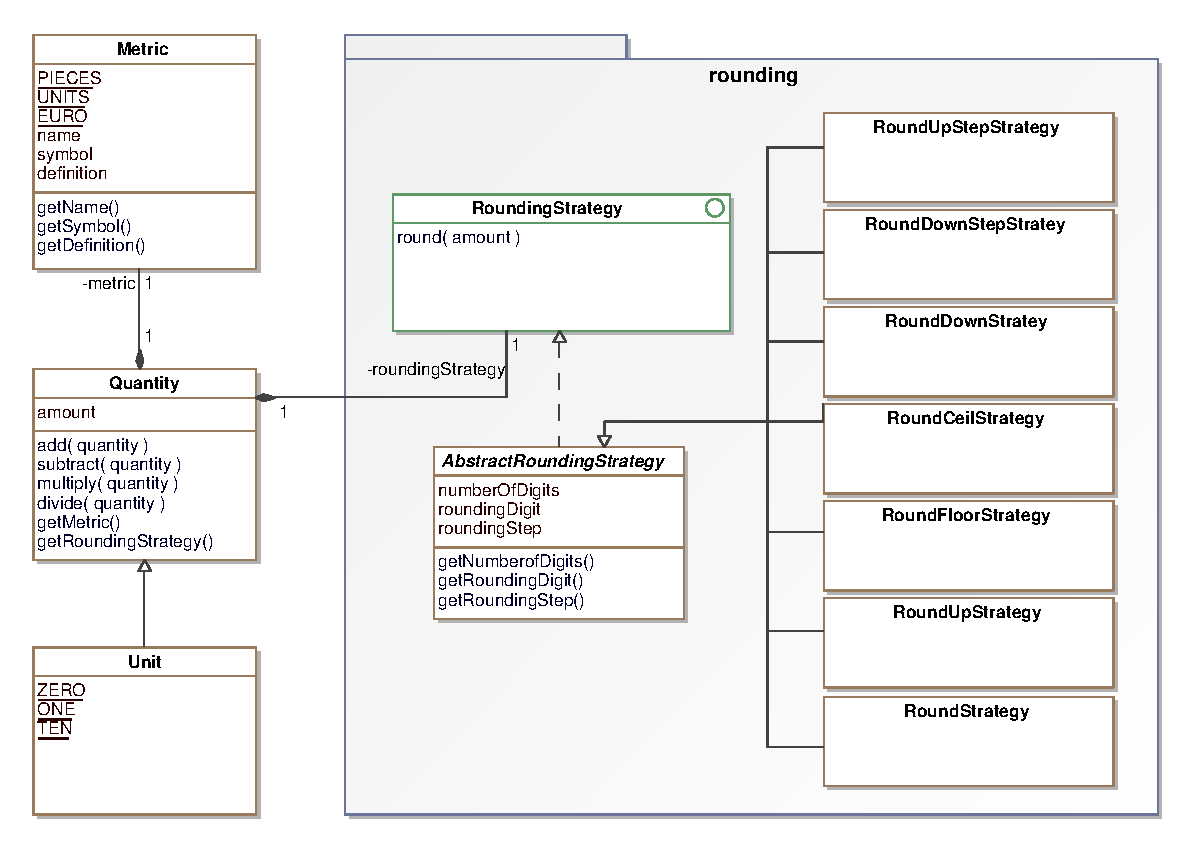
\includegraphics[width=1.0\textwidth]{images/Quantity_Overview.eps}
	\label{quantity_overview}
	\caption{Quantity - Class Overview}
\end{figure}

\subsection{\code{BigDecimal} - Representing numerical values}
\code{BigDecimal} was chosen over \code{float} or \code{double} because of its arbitraty precision.
Moreover, objects of \code{BigDecimal} are immutable and the \code{BigDecimal} class provides operations for including, but not limited to: arithmetic, rounding, and comparison.

\subsection{\code{Metric} - What is represented}
The composite type \code{Metric} contains all information pertaining to the unit or metric of the represented object.
Examples for units or metrics are: m (meter), s (second), pcs (pieces).
Thus, a metric can be described by a symbol (m) and a name (meter).
Furthermore, an object of type \code{Metric} has a description field, to explain the meaning of the metric in detail.

Convenience instances exist for euros, pieces and units.

\subsection{\code{RoundingStrategy} - How to handle half a person}
When handling quantities of unkown metric, standard rounding rules cannot always be employed.
The case of natural persons is just one example, when rounding rules have to be restricted to yield a useful result.
You can round in for general directions: away from zero, towards zero, towards positive infinity, and towards negative infinity.

Additionally, you can specify the digits after the decimal delimiter.
Monetary values in \euro{} or \$US are often just represented with two digits after the decimal delimiter.
Other values, such as kilo grams may be required to be specified to four digits after the decimal delimiter or even further.
In case of (natural) persons, the digits after the decimal delimiter is usually zero, except you are working in statistics (1.45 children per couple) or you are a serial killer dismembering your victims.

The third parameter for rounding is the rounding digit, i.e. the number specifying when you round up or down.
Usually, this number is five.
In case of persons, it is one: if you have $n.0\,persons$, you round down, otherwise up.
If you are calculation a capacity for persons, you will have to round down, this can be done by specifying the correct rouding direction.

Sometimes, it is necessary to round a number to a nearest ``step'', i.e. if you sell something in packs of $50$, and someone punches in $40$, you will have to round up to $50$.
So your rounding step is $50$.
Another example is material, which is sold by the meter or yard.
You have to round the amount specified by your customer accordingly.
Of course, a rouding step can be smaller than $1$, i.e. $0.25$.

Two convenience rounding strategies exist so far: \code{RoudingStrategy.MONETARY} rouding with four digits after the decimal delimiter and rouding towards zero, and \code{RoudingStrategy.ROUND\_ONE} with zero digits after the decimal delimiter and also rouding towards zero.

\subsection{\code{Money} - A usecase for \code{Quantity}}
Objects of class \code{Money} are used to represent amounts of currency within Salespoint.
The following paragraphs detail the intended use, internal modelling and implementation of \code{Money}.

\begin{figure}[ht]
	\centering
  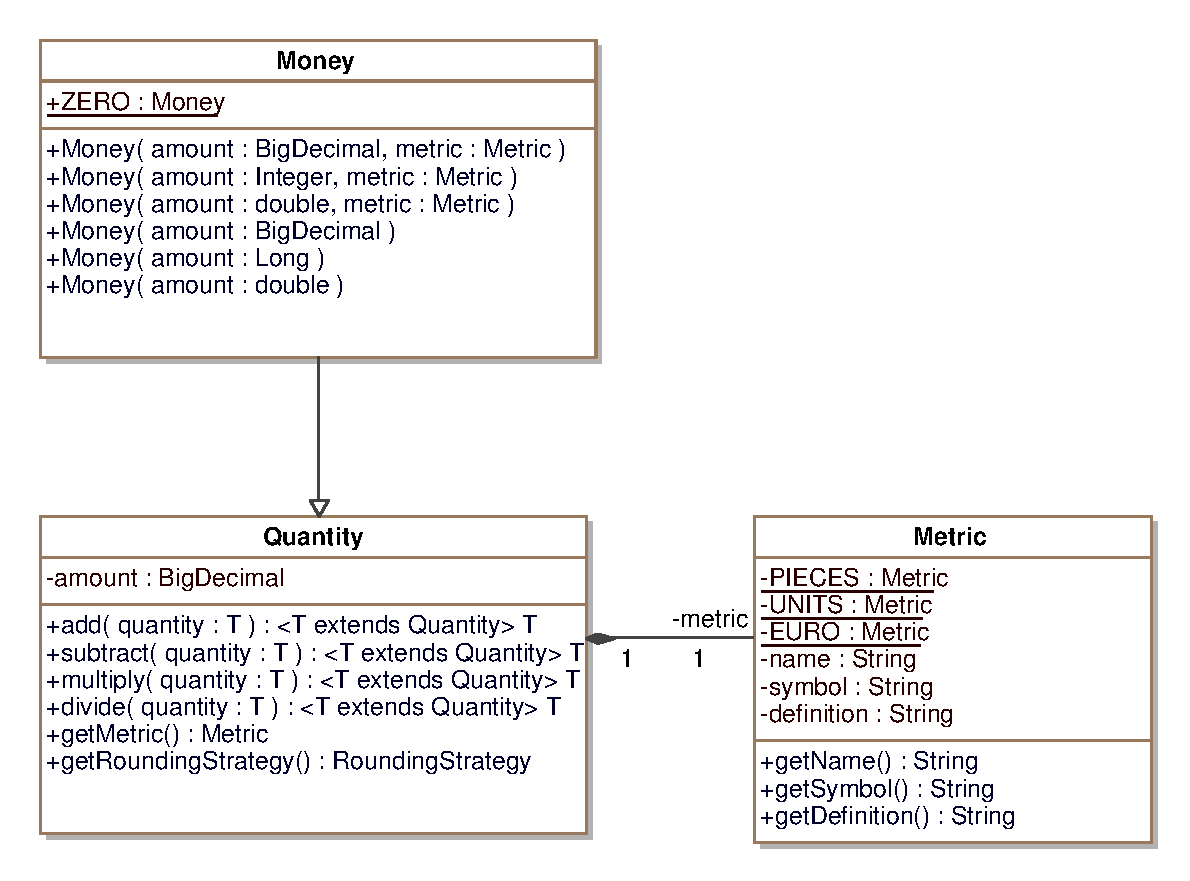
\includegraphics[width=1.0\textwidth]{images/Money_Overview.eps}
	\label{money_overview}
	\caption{Money - Class Overview}
\end{figure}

A \code{Money} object can be instatiated by just passing the numerical value as constructor parameter.
In this case, the metric \code{Metric.EURO} is used, as well as \code{RoundingStrategy.MONETARY} for the rounding strategy attribute.

For other currencies, a \code{Metric} parameter can be passed to the constructor along with a numerical paramter.
However, conversion between currencies is not supported, as is was not deemed necessary.

The rounding strategy cannot be overridden.

Internally, \code{Money} objects calculate with and are rounded to four digits after the decimal delimiter to minimize the rounding error.
The \code{toString()} method, however, limits the output to the expected two digits after the decimal delimiter and appends the symbol of the associated \code{Metric}.

Two convenience instances exist: \code{Money.ZERO}, representing \euro{0,00}, and \code{Money.OVER9000}, representing an amount greater than \euro{9000,00}.

\subsection{\code{Unit} - Representing persons or other integral items}
To represent integral items conveniently, the objects of class \code{Unit} can be used.
The rouding strategy is fixed for all instances to \code{RoundingStrategy.ROUND\_ONE} and \code{Metric.PIECES} is used as metric.
Convenience instances for amounts of zero, one and ten unit(s) exist (\code{Unit.ZERO}, \code{Unit.ONE}, and \code{Unit.TEN}).

\newpage
\section{Product}

Products are represented by ProductTypes.

\begin{figure}[ht]
	\centering
  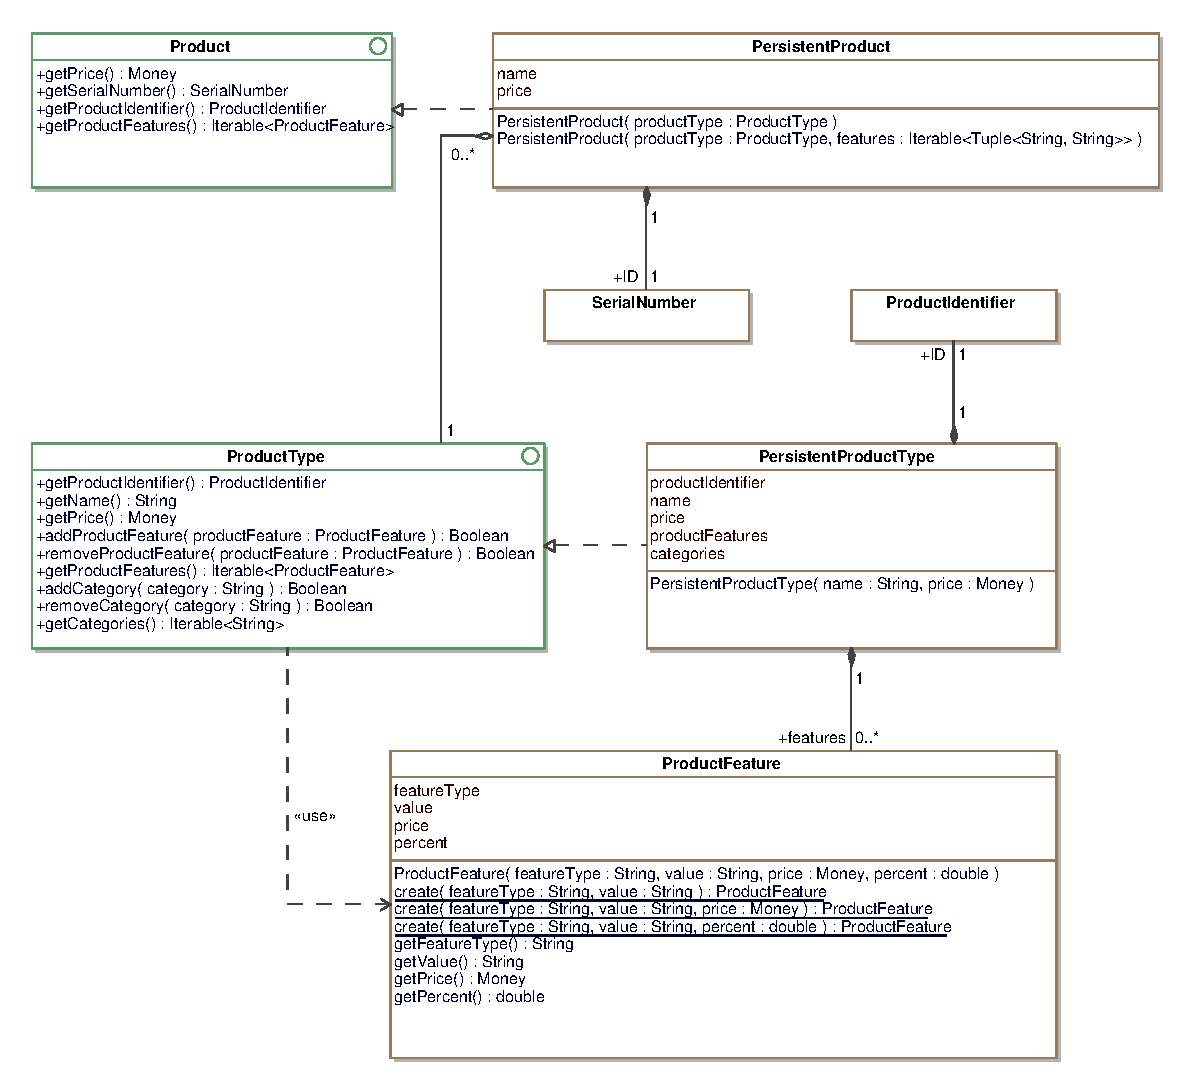
\includegraphics[width=1.0\textwidth]{images/Product_Overview.eps}
	\label{product_overview}
	\caption{Product - Class Overview}
\end{figure}

\subsection{\code{ProductType} - Representing specified products}
A \code{ProductType} is an interface which represents a specified product. The \code{AbstractProductType}-class is an implementation of this interface to worked with it.
An \code{AbstractProductType} contains a set of \code{ProductFeatureTypes} to specify your product. You can add any \code{ProductFeatureTypes}  to this set or remove them from it.
An example: Our specified \code{ProductType} is a table. About to sell any variations of this table, you need any \code{ProductFeatureTypes} like a corner table or a side table. 
So one \code{ProductFeatureType} represents one sort.

\subsection{\code{ProductFeatureType} and \code{ProductFeature} - Creating Features}
Every \code{ProductFeatureType} has a name, a description and a map of \code{ProductFeatures}, which define the \code{ProductFeatureType}. It's possible to add 
\code{ProductFeatures} to this map or remove them from it. So you can create your own \code{ProductFeatureType} with any \code{ProductFeatures}.\\
A \code{ProductFeature} can be for example a specified color or a special part of one or many products and has a name and a price.   

\subsection{\code{ProductInstance} - Representing ProductTypes}
A \code{ProductInstance} is an interface which represents one specified \code{ProductType}. The \code{AbstractProductInstance}-class is an implementation of this interface to worked with it.
If you create a \code{AbstractProductInstance}, it gets a \code{SerialNumber} and the \code{ProductIdentifier} of the \code{AbstractProductType} and the price will be calculated.
\code{SerialNumber} and \code{ProductIdentifier} are unique \code{SalespointIdentifier} to identify \code{ProductInstances} and \code{ProductTypes} in the database. 
Also you can add \code{ProductFeatures} to the \code{AbstractProductInstance}, which will be needed. Automatically the price of this \code{AbstractProductInstance} will be recalculated, 
so the price of these features will be added.\\
There are subclasses of \code{ProductType} and \code{ProductInstance}, with them the functionality will be extended. The subclasses of \code{ProductType} are \code{ServiceType} and 
\code{MeasuredProductType}, the subclasses of \code{ProductInstance} are \code{ServiceInstance} and \code{MeasuredProductInstance}. 

\subsection{\code{ServiceType} - Realizing Services}
The interface \code{ServiceType} is implemented by the class \code{AbstractServiceType}. With this class you can realize services in your implementation, which represents a process 
or activity that is offered for sale, for example a haircut on a barber shop or a driving lesson on a driving school.\\
Every \code{AbstractServiceType} has a name and a price and can contains a start time and an end time. Between these dates the \code{AbstractServiceType} can be executed. If these dates 
don’t exist, the \code{AbstractServiceType always} is offered.

\subsection{\code{ServiceInstance} - Representing ServiceTypes}
The interface \code{ServiceInstance} is implemented by \code{AbstractServiceInstance}, which represents one specified \code{AbstractServiceType}. The \code{AbstractServiceInstance} has a 
start time and an end time like its \code{AbstractServiceType}. The start time must be after the start time of \code{AbstractServiceType} and before the end time of 
\code{AbstractServiceInstance}. The end time must be before the end time of \code{AbstractServiceType}.\\
Otherwise it will be thrown exceptions:
\begin{itemize}
\item \code{IllegalArgumentException}: If the \code{ServiceInstance} end before it starts.
\item \code{IllegalArgumentException}: If the \code{ServiceInstance} begin before the period of \code{ServiceType} has begun.
\item \code{IllegalArgumentException}: If the \code{ServiceType} end after the period of \code{ServiceType} was finished.
\end{itemize}
Also you can cancelled the \code{AbstractServiceInstance} with the method \code{public void cancelServiceInstance()} and so the end time is now and you can get the 
\code{ServiceDeliveryStatus} of the \code{AbstractServiceInstance} at every time.
  
\subsection{\code{ServiceDeliveryStatus}}
The \code{ServiceDeliverystatus} is an enumeration with follow attributes:
\begin{itemize}
\item \code{SCHEDULED}: If the start of the \code{ServiceInstance} is in the future.
\item \code{EXECUTING}: If the \code{ServiceInstance} is executing now.
\item \code{CANCELLED}: If the \code{ServiceInstance} was cancelled.
\item \code{COMPLETED}: If the \code{ServiceInstance} is completed, so the end of the \code{ServiceInstance} is in the past and it wasn’t cancelled.
\end{itemize}

\subsection{\code{MeasuredProductType} - Creating MeasuredProducts}
The interface \code{MeasuredProductType} is implemented by \code{AbstractMeasuredProductType}. With this class you can realize products, which are not sold as predefined unit, but rather 
as measures of something. For example flooring may be sold by square foot or fresh products by kilogram.
A \code{AbstractMeasuredProductType} has a name, a price and a quantity on hand. The quantity on hand, is the quantity of this \code{AbstractMeasuredProductType}, which is available to 
be sold. You can also add or reduce a specified quantity of the \code{AbstractMeasuredProductType} to it. 
The price of the \code{AbstractMeasuredProductType} isn’t the price for an unit of that, but the price of the quantity on hand of that. The unit price will be calculated automatically 
and you can get it with the method \code{getUnitPrice()}.

\subsection{\code{MeasuredProductInstance} - Representing MeasuredProductTypes}
The interface \code{MeasuredProductType} is implemented by \code{AbstractMeasuredProductType}, which represents a specified quantity of the \code{AbstractMeasuredProductType}. If it’s 
created, the quantity of that, will be reduce from the quantity on hand of the \code{AbstractMeasuredProductType}, because this quantity is used and no more available for other 
\code{AbstractMeasuredProductInstances}. If this quantity is greater than the quantity on hand, an exception will be thrown.
\newpage
\section{Catalog}

\begin{figure}[ht]
	\centering
  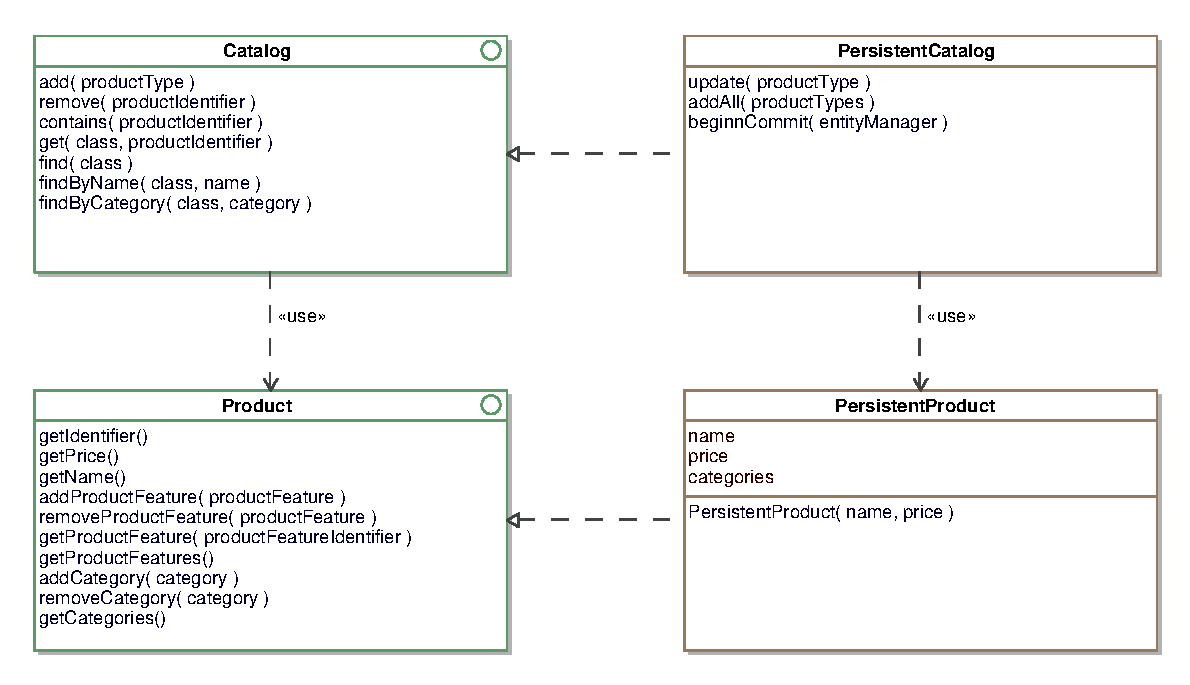
\includegraphics[width=1.0\textwidth]{images/Catalog_Overview.eps}
	\label{catalog_overview}
	\caption{Catalog - Class Overview}
\end{figure}

\subsection{\code{Catalog} - Organizing and presenting \code{ProductTypes}}
\code{Catalog} is an interface and provides methods for adding and removing \code{ProductTypes} as well as finding them based on the \code{ProductType} via its name and category.
\code{PersistentCatalog} is an implementation of the \code{Catalog}-interface and provides the \code{update(PersistentProductType productType)} method for updating and persisting an existing \code{PersistentProductType} to the \code{PersistentCatalog} and the database. 
Every operation is delegated to the database, via \code{CriteriaQuery}s. Some methods require additional processing of query results with Java.
\code{Catalog} aggregates \code{ProductType}s, \code{PersistentCatalog} aggregates \code{PersistentProductType}s.




%If you want to sell your products at your shop, you must presenting them very good to stimulate customers interests. A helpful solution to giving this people a clearly overview could be
%a catalog. With the \code{PersistentCatalog}-class, you can implemented such a thing. This class is an implementation of the interface \code{Catalog}.\\
%After you created a new catalog, you can add \code{ProductTypes} to it or remove them from it. Also you can checked, whether the catalog contains a defined \code{ProductType}. Aside from you 
%this class provides methods to find productTypes by their name or their category at your catalog.\\
%In case you have added a \code{ProductType} to the catalog and now you are changing this type, you do not need remove the old type from this catalog and add the new to it. Only you need to 
%used the method \code{update(PersistentProductType productType)} from the \code{PersistentCatalog}-class and this \code{productType} will be updated and persist to the \code{PersistentCatalog} 
%and the Database.


\section{Inventory}
\label{sec:inventory}

\begin{figure}[ht]
	\centering
  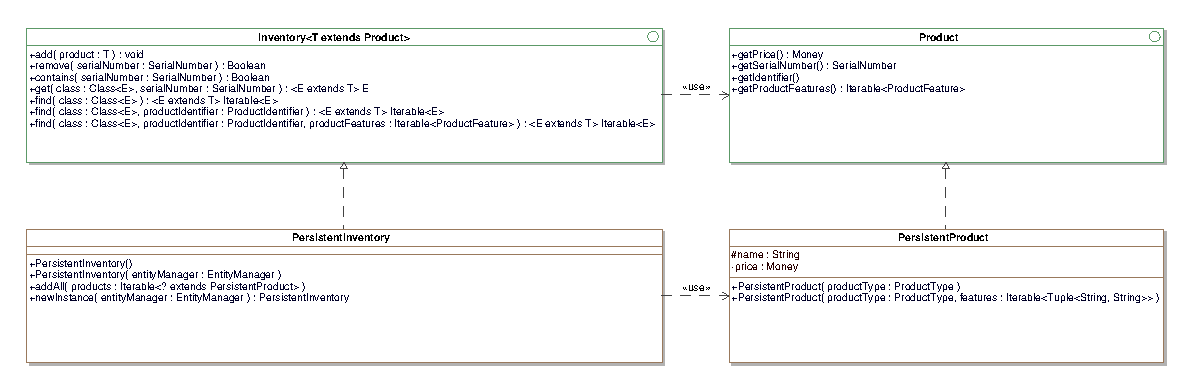
\includegraphics[width=1.0\textwidth]{images/Inventory_Overview.eps}
	\label{inventory_overview}
	\caption{Inventory - Class Overview}
\end{figure}

An inventory is a place, where products are stored.
In \salespoint{}, an abstract representation if the \code{Inventory} interface and its implementing class \code{PersistentInventory}.
The interface and declares methods to add, remove and find products.
Because an inventory contains specific product instances, \code{PersistentInventory} aggregates \code{PersistentProductInstance}s.

\code{PersistentProductInstance}s can be retrieved from \code{PersistentInventory} by specifying a \code{SerialNumber} or a \code{ProductIdentifier}.
A \code{SerialNumber} is used to reference a specific \code{ProductInstance}.
A \code{ProductIdentifier} identifies a \code{Product} uniquely, thus all \code{PersistentProductInstance}s of the \code{PersistentProduct} specified by the supplied \code{ProductIdentifier} are returned.
Additionally an \code{Iterable<ProductFeature>} can be supplied to the \code{find()}-method along with a \code{ProductIdentifier} to retrieve all instances of a product, where the \code{ProductFeature}s match exactly those specified.
Matching a set of \code{ProductFeatures} against a \code{PersistentProductInstance} is hard to express in JPQL or Criteria Queries.
Therefore, only the \code{ProductIdentifier} is used to build a Criteria Query, which is executed on the database.
Selecting only those \code{PersistentProductInstances} which match the specified \code{ProductFeature}s is done in Java code.
%\code{Inventory} aggregates \code{Product}s, \code{PersistentInventory} aggregates \code{PersistentProduct}s 

%A shop must store products in an inventory, because the customer should get your good on order very quickly. If there are no amount of this product inside, it must be ordered by its producer.
%This procedure can be implemented by the \code{PersistentInventory}-class. This class is an implementation of the interface \code{Inventory}, to used its functionality and also 
%to persist the items of your inventory.\\
%With the methods of the \code{Inventory}-class you can add one or many \code{Products} to the inventory, you can remove a product from it or you can checked, whether a product exist in it.
%Also you can find \code{Products} with several options, if you know the \code{ProductIdentifier}, their \code{productFeatures} or the classes of them.

\newpage
\section{Accountancy}
The accountancy package contains functionality pertaining to book keeping.
As in other packages, interfaces are used to separate between behaviour and implementation.
\code{AccountancyEntry} is a representation of an accounting entry.
\code{Accountancy} aggregates \code{AccountancyEntry}s.
By implementing and subclassing \code{AccountancyEntry} the notion of different accounts, as known from double-entry bookkepping, can be realised.
Every \code{AccountancyEntry} is uniquely identified by an \code{AccountancyEntryIdentifier}.
\\

\code{PersistentAccountancyEntry} implements \code{AccountancyEntry} and serves as persistence entity, while \code{PersistentAccountancy} implements \code{Accountancy} and provides opaque access to the JPA layer.
\code{AccountancyEntryIdentifier} is used as primary key attribute, when persisting entities to the database.
\\

As can be seen in Figure \ref{accountancy_overview}, \code{PersistentAccountancyEntry} is sub classed to create a second ``account'' used to store payment information, namely \code{ProductPaymentEntry}.
To access entries of only one type, thus belonging to one ``account'', \code{get()} and \code{find()} methods in \code{Accountancy} have a type parameter.

Payment information also includes a user identifier referencing the buyer, an order identifier referring to the \code{Order} which was payed, and a \code{PaymentMethod} describing the money transfer.
The inheritance hierarchy of \code{PaymentMethod} is depicted in Figure \ref{payment_overview}.
\begin{figure}
	\centering
  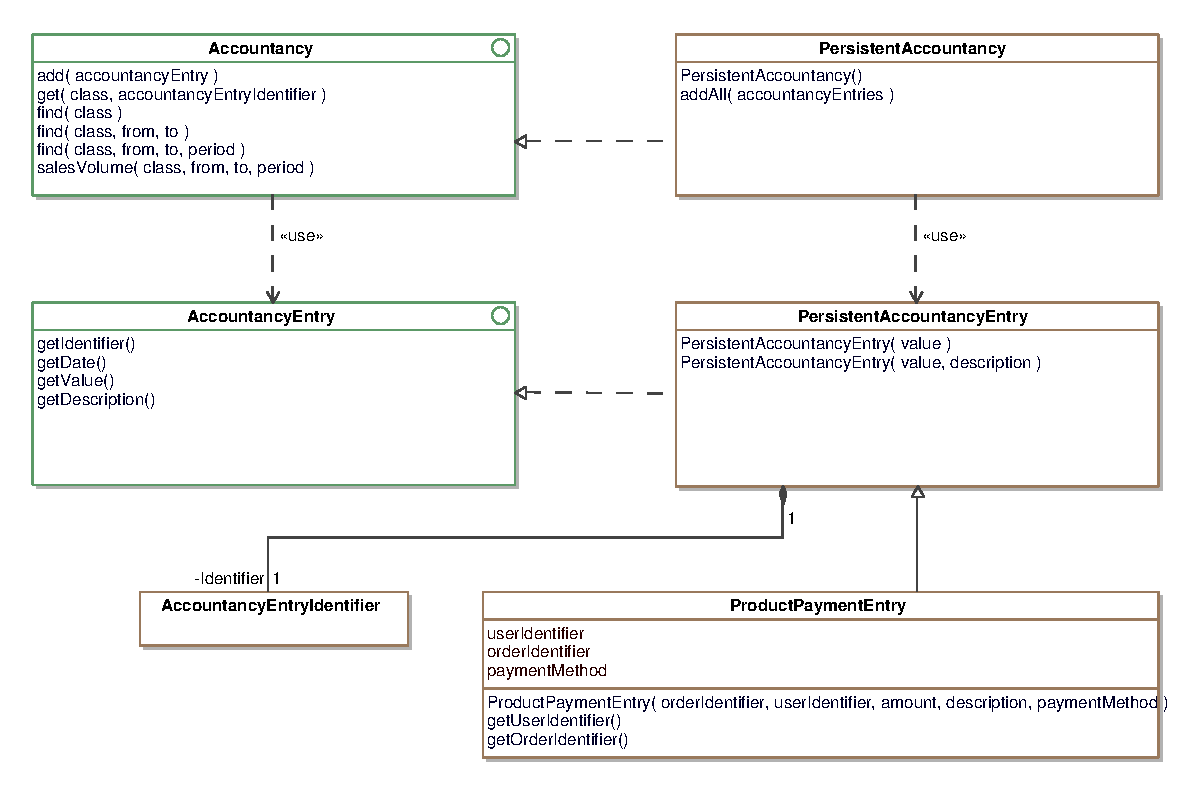
\includegraphics[width=1.0\textwidth]{images/Accountancy_Overview.eps}
	\label{accountancy_overview}
	\caption{Accountancy - Class Overview}
\end{figure}

\begin{figure}
\centering
  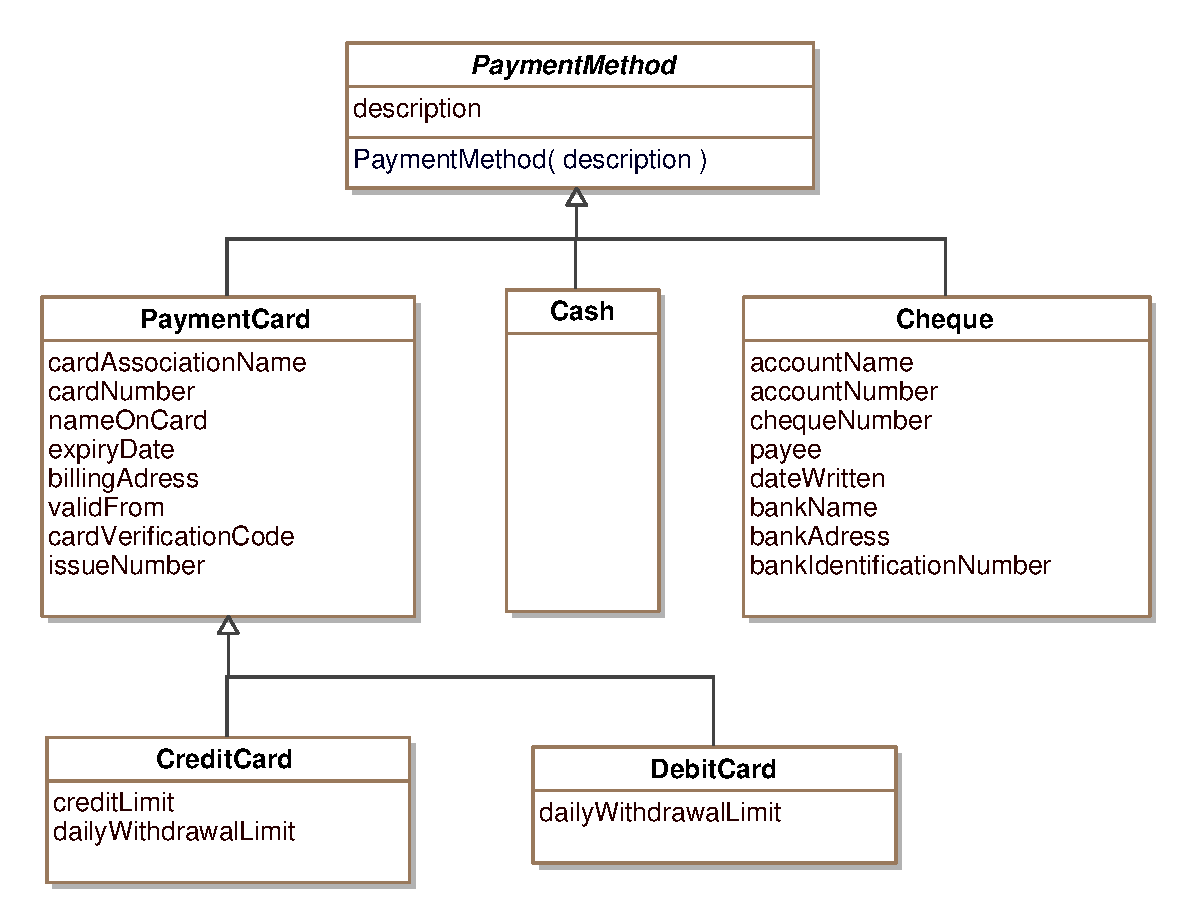
\includegraphics[width=1.0\textwidth]{images/Payment_Overview.eps}
	\label{payment_overview}
	\caption{Payment - Class Overview}
\end{figure}

\newpage
\section{Order}
Orders are a new feature in Salespoint 2011. The intention was to prepare the old databaskets for development of web applications and extend them to collaborate with our new inventory, providing the opportunity of individual pricing, final payment and basic log functionality.

\begin{figure}[ht]
	\centering
  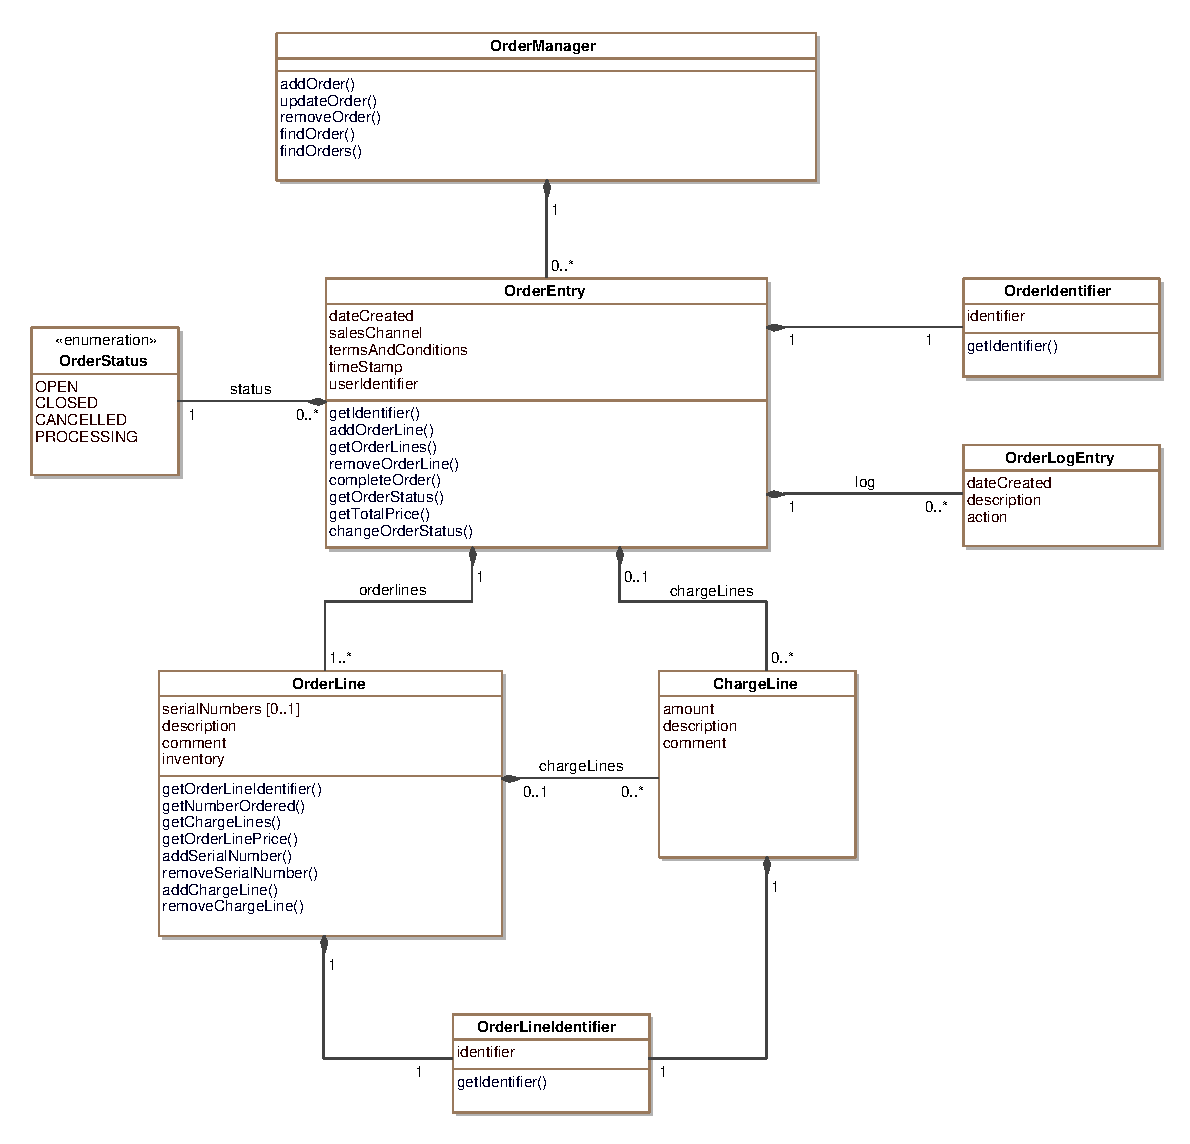
\includegraphics[scale =.7]{images/Overview_Order.eps}
	\label{order_overview}
	\caption{Order - Class Overview}
\end{figure}

\subsection{\code{OrderEntry} - The main data structure}
We created the \code{OrderEntry} as main data structure to access the functionality above. An \code{OrderEntry} represents one order and can be imagined as sheet of paper which basically consists of lines representing the ordered products (\code{OrderLine}) and lines that are not bound to a concrete product but which cause charge (\code{ChargeLine}). \code{ChargeLines} make it possible to add individual charge to orders. For example they can be used to define forwarding charges or other special charges produced by this order. 

\code{OrderEntrys} are lifecycle-objects. The lifecycle covers four states which are defined by enumeration type \code{OrderEntryStatus}. After all the lifecycle has no restrictions in changing states with one exception: \code{CLOSED} is a final state and it's not possible to change the state of \code{CLOSED} \code{OrderEntrys}. The state machine below shows an example of a frequently practised lifecycle.

\begin{figure}[ht]
	\centering
  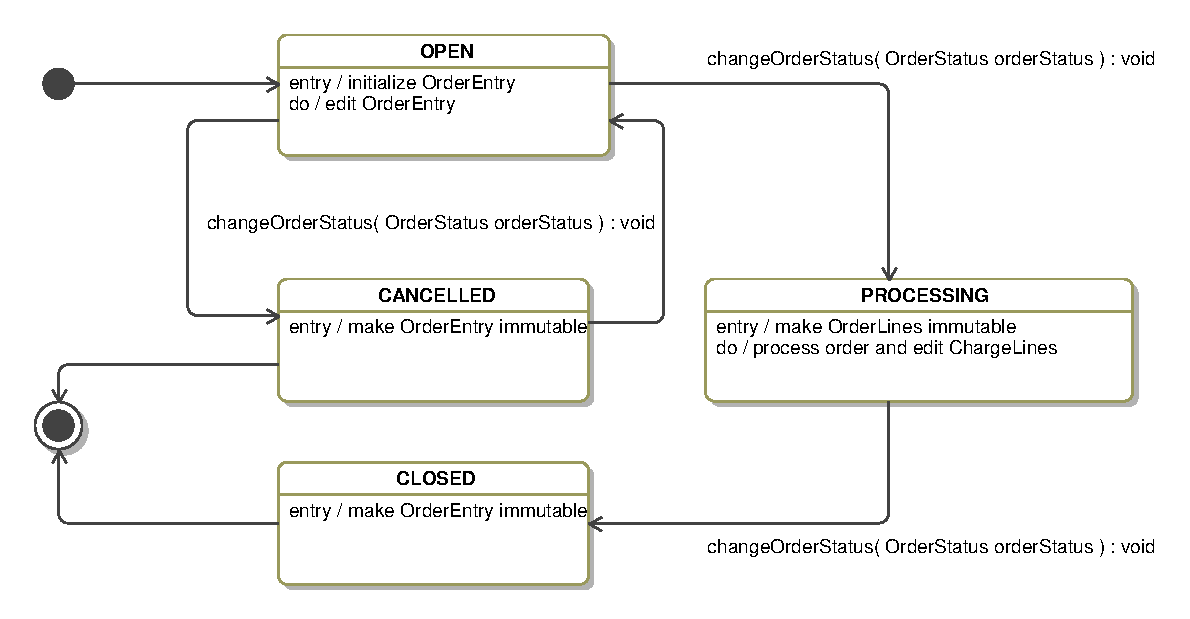
\includegraphics[scale =.7]{images/OrderEntryState.eps}
	\label{order_statemachine}
	\caption{Order - Lifecycle}
\end{figure}  

As you can see an OrderEntry can only completely modified in state \code{OPEN}. \code{CANCELLED} and \code{CLOSED} \code{OrderEntrys} are immutable! \code{PROCESSING} \code{OrderEntrys} are basically also immutable but their is still the possibility to modify the \code{ChargeLines} of that \code{OrderEntrys}. 

\subsection{\code{OrderLine} - Representing ordered objects}
An \code{OrderLine} contains all information needed to identify product instances and deal with them. Every \code{OrderLine} is mapped to an \code{Inventory} and contains all \code{Serialnumbers} that are ordered from this \code{Inventory}. Hence an \code{OrderEntry} can contain as far \code{OrderLines} as \code{Inventories} exist. If two or more \code{OrderLines} from same \code{Inventory} will be added to an \code{OrderEntry}, they will be automatically merged into one \code{OrderLine}.
As well as \code{OrderEntrys}, \code{OrderLines} can also contain \code{ChargeLines}. Notice that these \code{ChargeLines} cannot be modified if the \code{OrderLine} is in context of an \code{CANCELLED} or \code{CLOSED} \code{OrderEntry}! 

\subsection{\code{ChargeLine} - Representing additional charge}
A \code{ChargeLine} represents an additional charge for an \code{OrderLine} over and above the \code{OrderLine} value or an extra charge added to an \code{OrderEntry}.

\subsection{\code{OrderManager} - The interface to JPA}
To simplify the management of \code{OrderEntries} we have implemented the \code{PersistentOrderManager}. With \code{PersistentOrderManager} you can persist, update, find and remove \code{OrderEntries}. \code{PersistentOrderManager} are non-Entity classes and cannot be persisted! Multiple \code{OrderManager} in the system working on the same database so it's possible to use seperate \code{PersistentOrderManager} for different tasks, if the functionality is needed.


\chapter{Collaboration}

The \salespoint{} framework is more than just a collection of classes and interfaces. It provides also processes between packages that are triggered automatically and ensure consistent work. This chapter gives attention to that dependencies between packages and describes how they collaborate.  

Figure \ref{package_overview} illustrates the main dependencies between \salespoint{} packages. As can be seen nearly all packages are interdependent.\\ 

The central class that connects all features in \salespoint{} is the \code{Shop}. The most packages access this class to communicate with other packages. Therefore the \code{Shop} contains all interfaces which are global connected. This class should also be the first point for software engineers to request the seperate regions of \salespoint{}.\\

Another package that collaborates with nearly all packages is the \code{Order} package. \code{OrderLines} using interfaces from \code{Product} package to identify product instances and calculate their prices. The \code{Catalog} package is used to check whether the catalog contains added products. \code{Orders} are also associated with the \code{UserManager}, to receive information about involved users.\par 
Completed \code{Orders} will communicate with the \code{Inventory} (via \code{Shop} class) to remove considered product instances. \par
Before completion, \code{Orders} have to be payed. An \code{Order} which changed its status to \code{PAYED} will automatically access the accountancy and create the corresponding \code{AccountancyEntry} which represents that payment.\\ 

\code{Catalogs} and \code{Inventorys} also work closely together with all classes in \code{Product} package. There are a lot of other packages and classes that provide structures which are used in \salespoint{} like the \code{Money} and \code{Quantity} packages. After all there are much more smaller collaborations in \salespoint{}, but the above described are the most important ones.







\clearpage
\phantomsection
\addcontentsline{toc}{chapter}{Bibliography}
\bibliographystyle{alpha}
\bibliography{bib}

\end{document}
